74. $y=\cfrac{2x-3}{|x+2|}=\begin{cases}\cfrac{2x-3}{x+2},\ x>-2,\\ \cfrac{2x-3}{-x-2},\ x<-2.\end{cases}=
\begin{cases}2-\cfrac{7}{x+2},\ x>-2,\\ -2+\cfrac{7}{x+2},\ x<-2.\end{cases}$
$$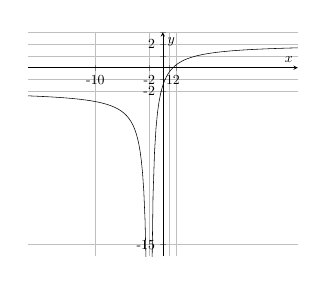
\begin{tikzpicture}[scale=0.5]
\begin{axis}[
    axis lines = middle,
    grid=major,
    legend pos={south west},
    xlabel = {$x$},
    %xlabel style={below right},
    ylabel = {$y$},
    ymin=-16,
    ymax=3,
    xmin=-20,
    xmax=20,
    xtick={-2,1,2,-10},
    xticklabels={-2,1,2,-10},
    ytick={-15,-2,-1,1,2,3},
    yticklabels={-15,-2,$ $,$ $,2,$ $},
                  ]
	\addplot[domain=-20:-2.1, samples=100, color=black] {(2*x-3)/abs(x+2)};
    \addplot[domain=-1.9:20, samples=100, color=black] {(2*x-3)/abs(x+2)};
        %\addplot[domain=2.01:6, samples=100, color=black] {2/(2-x)};
   % \addplot[domain=-3:3, samples=100, color=black] {-x};
     %\addlegendentry{$\text{Рис. 1}$};
\end{axis}
\end{tikzpicture}$$
